\documentclass[a4paper, 10pt]{article}

\usepackage[utf8]{inputenc}
\usepackage[main=ngerman, english, russian]{babel}  % titles & autogenerated content in german
\usepackage{graphicx}
\usepackage{blindtext}
\usepackage{amssymb}
\usepackage{amsmath}
\usepackage{amsfonts}
\usepackage{xcolor}
\usepackage{csquotes}
\usepackage{pgfplots}
\usepackage[export]{adjustbox}
\usepackage[pages=some]{background}
\usepackage[a4paper, voffset = 20pt, textheight = 670pt]{geometry}

\newcommand{\xone}{-97}
\newcommand{\xtwo}{97}
\newcommand{\yone}{7}
\newcommand{\ytwo}{-275} % for pdf: -275, for printing: -273

\usepackage{hyperref}  % clickable links in PDF
\hypersetup{
    colorlinks   = true,    % Colours links instead of ugly boxes
    urlcolor     = blue,   % Colour for external hyperlinks
    linkcolor    = black,   % Colour of internal links
    citecolor    = black
}

\usepackage[
    %style=authoryear-comp
    style=numeric-comp,
    %style=verbose
    sorting=none,
]{biblatex}
\addbibresource{sources.bib}

\addto\captionsngerman{\renewcommand*\contentsname{Inhalt}}
\addto\captionsngerman{\renewcommand*\abstractname{Abstract}}

\newcommand{\comment}[1]{} % multiline comment

\graphicspath{ {./images/} }

\title{
    \vspace{-2em}
    \Large CT projekt \\
    %\vspace{0.5em}
    \rule{\linewidth}{1pt}
    \textsc{
    \huge Raytracing \\
    }
    \rule{\linewidth}{1pt}
}
\author{Christian Korn, TGI 13/4}
\date{SJ2022-2023 H2} % Ende: TBD

%%%%%%%%%%%%%%%%%%%%%%%%%%%%%%%%%%%%%%%%%%%%%%%%%%%%%%%%%%%%%%%%%%%%%%%%%%%%%%%%%%%%%%%%%%%%%%%%%%%%%%%%%%%%%%%%%%%%%%%%

\begin{document}

\newgeometry{total={170mm, 270mm}, voffset = 0pt}
\begin{titlepage}
    \backgroundsetup{contents={
        \includegraphics[]{images/title_image.png}},
        angle=0,
        scale=0.2,
        %hshift=3.5cm,
        %vshift=-0.5cm,
        opacity=1
    }
    \BgThispage
   
    \centering{
    \vspace{30cm}
    \begin{tikzpicture}[overlay] % White border around the page
        \draw[white, ultra thick]  
            (\xone mm, \yone mm)
         -- (\xtwo mm, \yone mm)
         -- (\xtwo mm, \ytwo mm) 
         -- (\xone mm, \ytwo mm)
         -- (\xone mm, \yone mm + 0.9pt); % additional length to fill the gap in the corner
    \end{tikzpicture}

    %\vspace{0.5cm}
    \color{white}
    \LARGE
    CT Projekt \\
    %\vspace{0.5cm}
    \rule{\linewidth}{1.5pt}
    \textsc{
    \Huge Raytracing \\
    }
    \vspace{-4pt}
    \rule{\linewidth}{1.5pt} \\
    %\vspace{19.7cm}
    \vspace{22cm}
    \Large
    Christian Korn

    }

\end{titlepage}
\restoregeometry

\maketitle

\begin{center}
    Der Quellcode kann unter 
    \href{https://github.com/MacAphon/RT}{https://github.com/MacAphon/RT} gefunden werden. 
\end{center}

%\tableofcontents

%\newpage

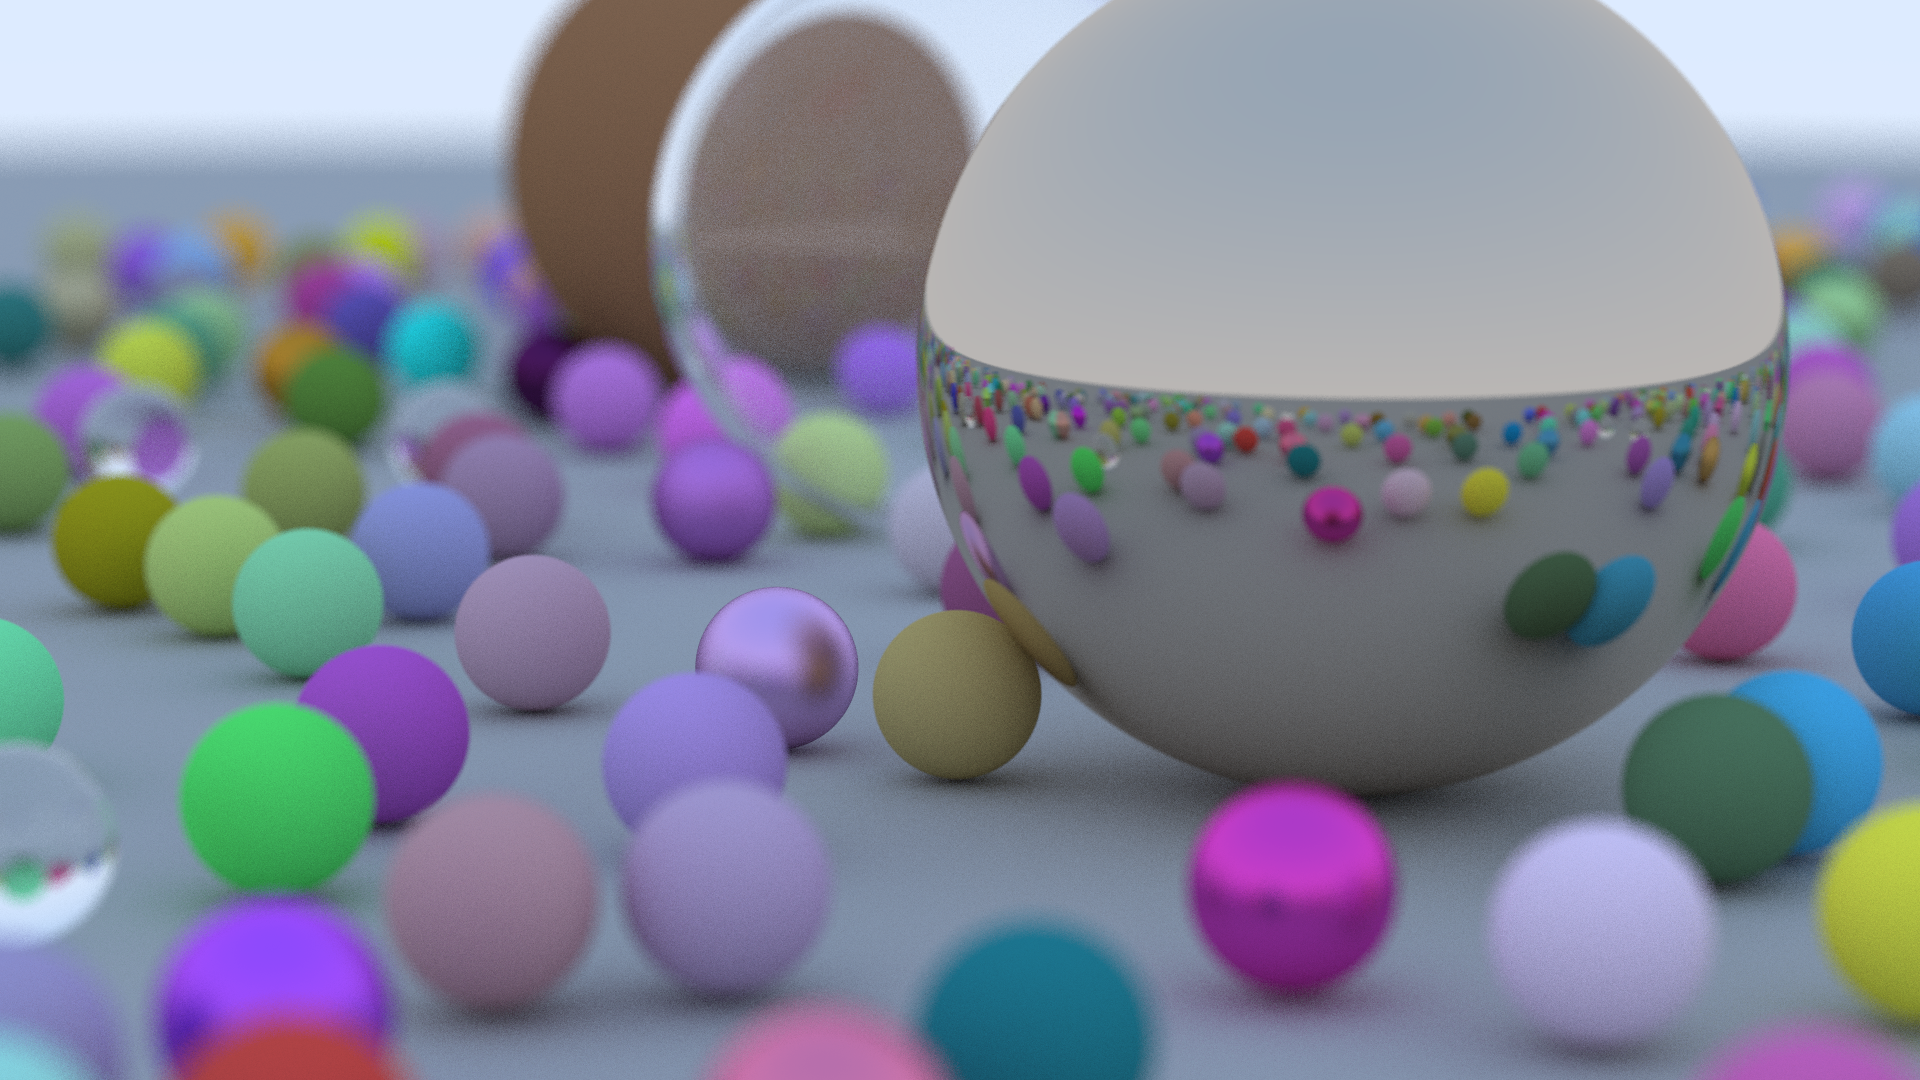
\includegraphics[scale=0.2]{images/large_scene.png}

\section{Projektidee}

Raytracing ist eine Technik zur Erstellung von Bildern, die auf der Simulation von Licht basiert.
Dabei wird für jeden Pixel des Bildes ein (oder mehrere) Strahlen in die Szene geschickt und die Farbe des Pixels anhand der Objekte, die der Strahl trifft, berechnet.
Durch die Simulation von Licht können realistische Bilder erstellt werden, die sich von Bildern, die mit Rasterisierung erstellt wurden, unterscheiden.

Dieses Projekt orientiert sich an Peter Shirley's Buch \enquote{Ray Tracing in One Weekend} \cite{Shirley2020RTW1}.
Teile des Codes orientieren sich außerdem an den Büchern \enquote{Ray Tracing: The Next Week} \cite{Shirley2020RTW2} und \enquote{Ray Tracing: The Rest of Your Life} \cite{Shirley2020RTW3}.

\section{Ziele}

\subsection{Verbindlich}

\begin{itemize}
    \item Erstellen von Bildern durch Raytracing
    \item Mehere darstellbare Objekte
    \item Verschiedene Materialien
\end{itemize}

Alle verbindlichen Ziele wurden erreicht.

Es sind vier verschiedene Materialien implementiert:
\begin{itemize}
    \item Lambertian (Matte Oberfläche)
    \item Metallisch (mit anpassbarer Rauheit)
    \item Dielektrikum (Glas, mit anpassbarem Brechungsindex)
    \item Emission
\end{itemize}
Bei allen Materialien kann die Farbe angepasst werden.

\subsection{Optional}

\begin{itemize}
    \item Transparenz mit Lichtbrechung
    \item Multithreading
    \item Verschiedene Ausgabeformate
    \item Lichtquellen
    \item Verschiedene Objekttypen
    \item Lesen der Szene aus Dateien
    \item Optimierungen 
\end{itemize}

\subsubsection*{Transparenz mit Lichtbrechung}

Die Transparenz mit Lichtbrechung wurde implementiert.
Zusätzlich wurde eine gute Approximation von Spiegelung bei spitzen Winkeln implementiert.

\subsubsection*{Multithreading}

Das Programm nutzt einen Threadpool, um die Berechnung der Pixel zu parallelisieren.
Die Anzahl der Threads kann über die Kommandozeile angegeben werden.

\subsubsection*{Verschiedene Ausgabeformate}

Das programm kan Bilder in den meisten gängigen Bildformaten ausgeben.

\subsubsection*{Lichtquellen}

Das Programm unterstützt Lichtquellen.
Bei jedem Auftreffen eines Strahls auf ein Objekt wird ein Zusätzlicher Strahl in Richtung der nächsten Lichtquelle geschickt.

\subsubsection*{Verschiedene Objekttypen}

Das Ziel wurde nicht erreicht, da nur Kugeln implementiert wurden.
Die Architektur des Programmes erlaubt aber die Implementierung weiterer Objekttypen ohne großen Aufwand.

\subsubsection*{Lesen der Szene aus Dateien}

Das Ziel wurde nicht erreicht, die Szene muss im Code erstellt werden.

\subsubsection*{Optimierungen}

Das Programm ist nicht optimiert.
Es gibt aber einige Optimierungsmöglichkeiten, die in Zukunft implementiert werden könnten, wie z.B.
Axis-Aligned Bounding Boxes.

\section{Beispielbilder}

\begin{minipage}[t]{0.5\linewidth}
    \centering
    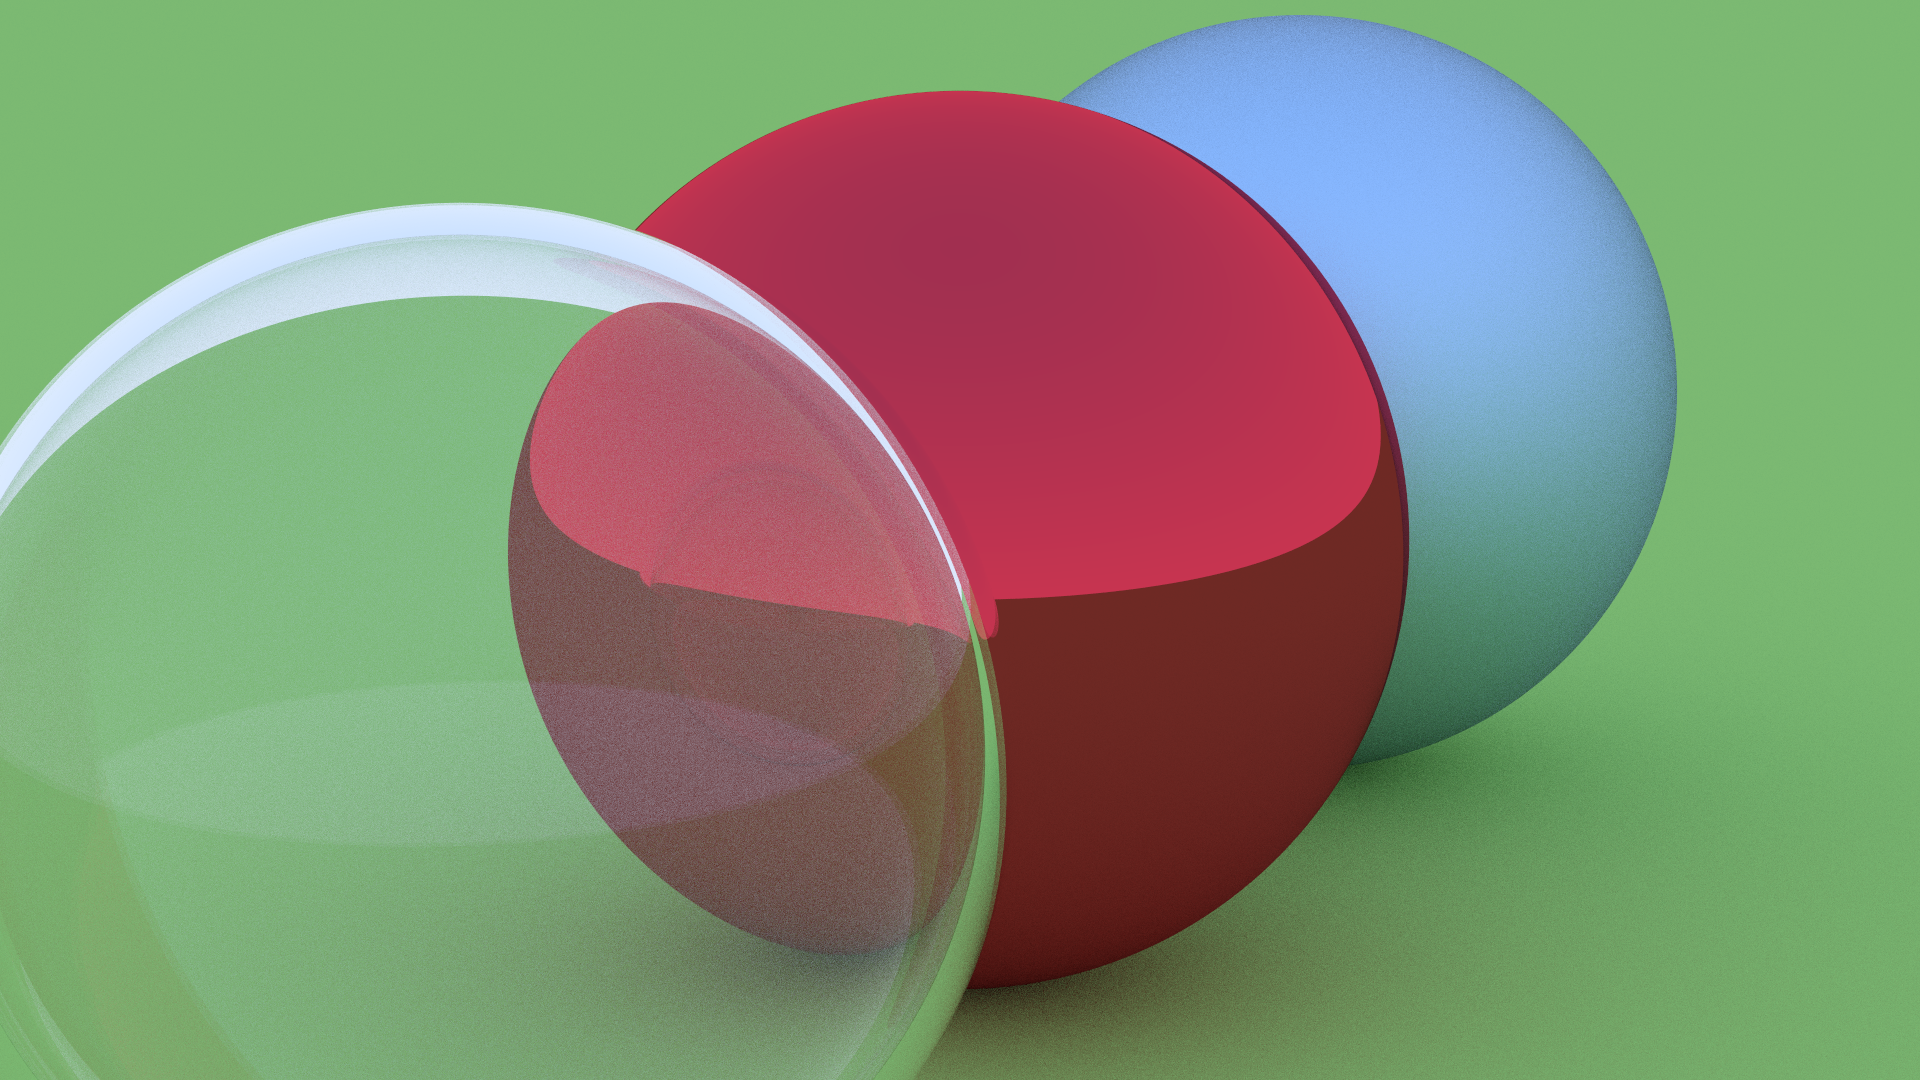
\includegraphics[width=\linewidth]{images/multiple_objects.png}
    Mehere Objekte mit verschiedenen Materialien

    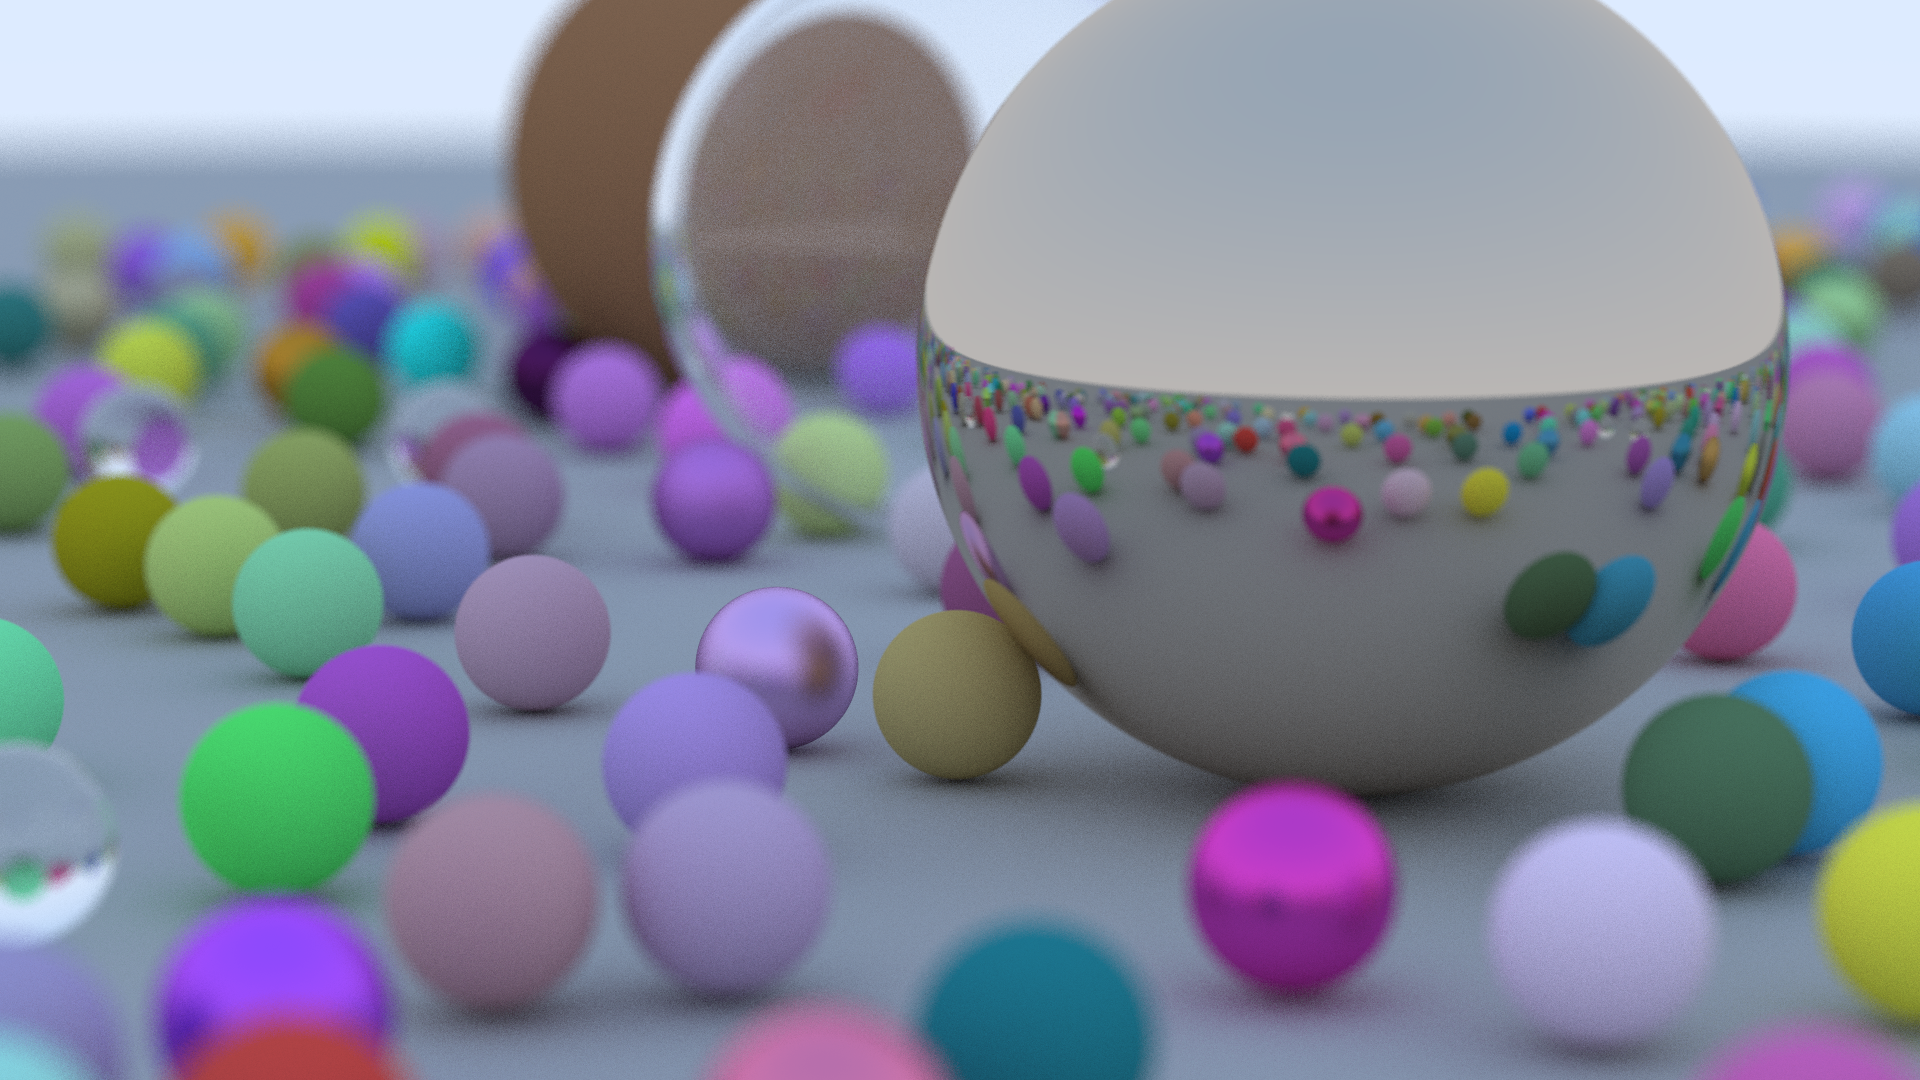
\includegraphics[width=\linewidth]{images/large_scene.png}
    Große Szene mit vielen Objekten

\end{minipage}
\begin{minipage}[t]{0.5\linewidth}
    \centering
    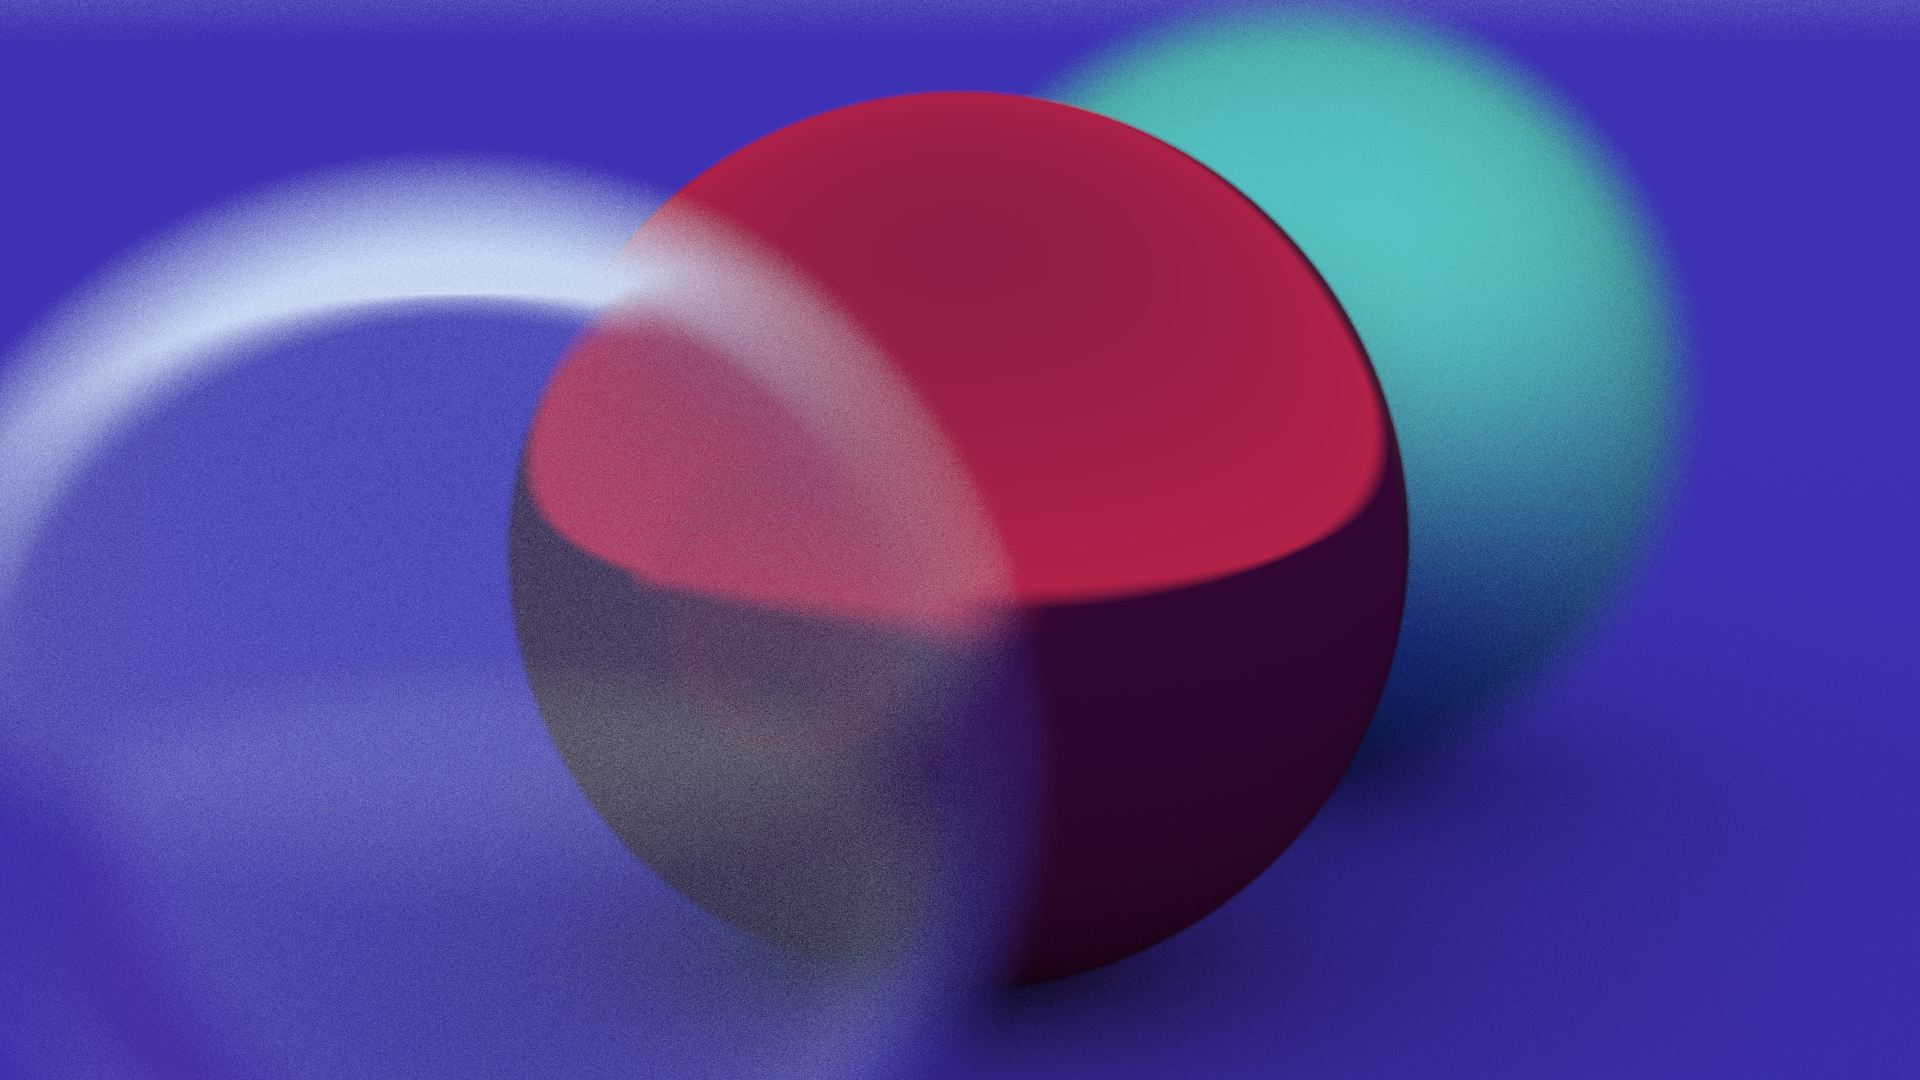
\includegraphics[width=\linewidth]{images/blur.png}
    Tiefenschärfe

    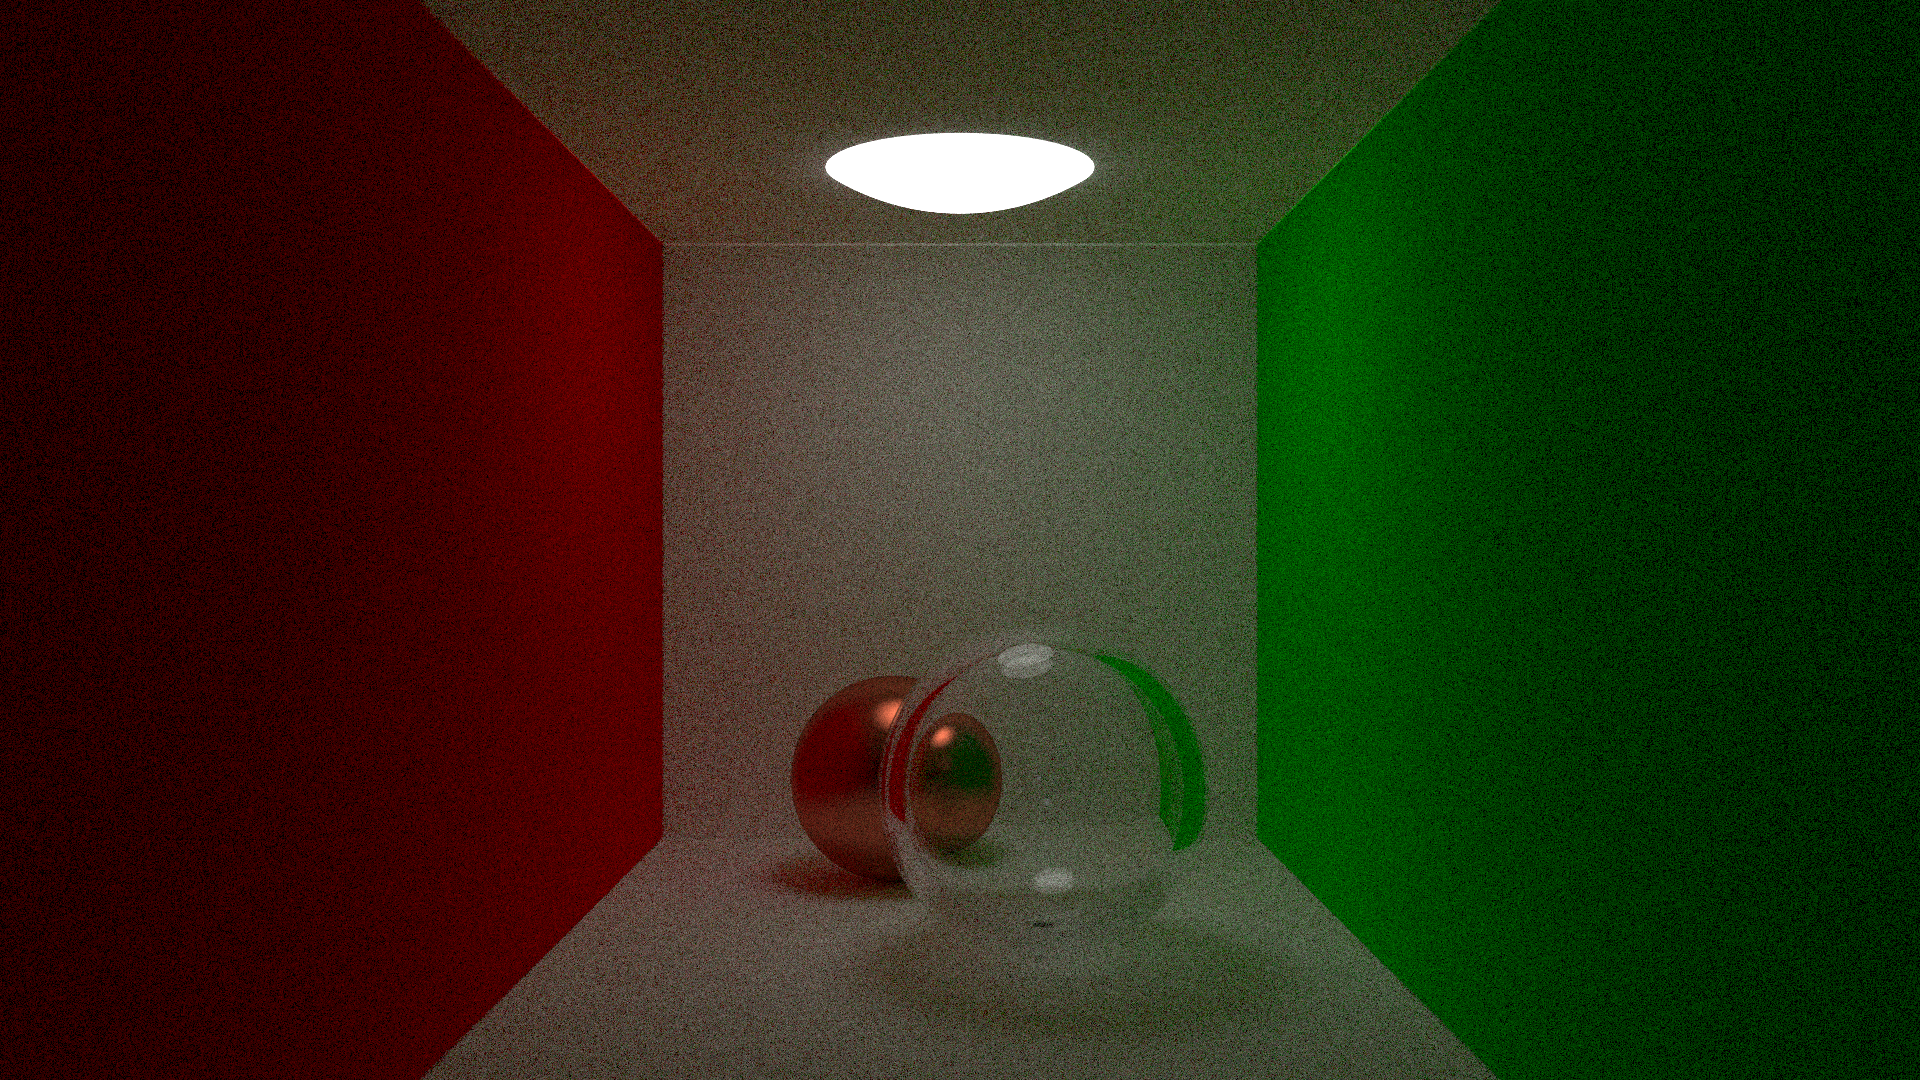
\includegraphics[width=\linewidth]{images/cornell.png}
    Cornell Box mit Lichtquellen

\end{minipage}

Für den Effekt einer hohlen Glaskugel wird in die Glaskugel eine zweite, kleinere Kugel gelegt.
Die kleinere Kugel hat den gleichen Brechungsindex wie die größere, hat aber einen negativen Radius.
Alternativ kann auch der inverse Brechungsindex der äußeren Kugel verwendet werden.

\section{Vergleich mit Blender}

\begin{center}
\begin{minipage}[b]{0.45\linewidth}
    \centering
    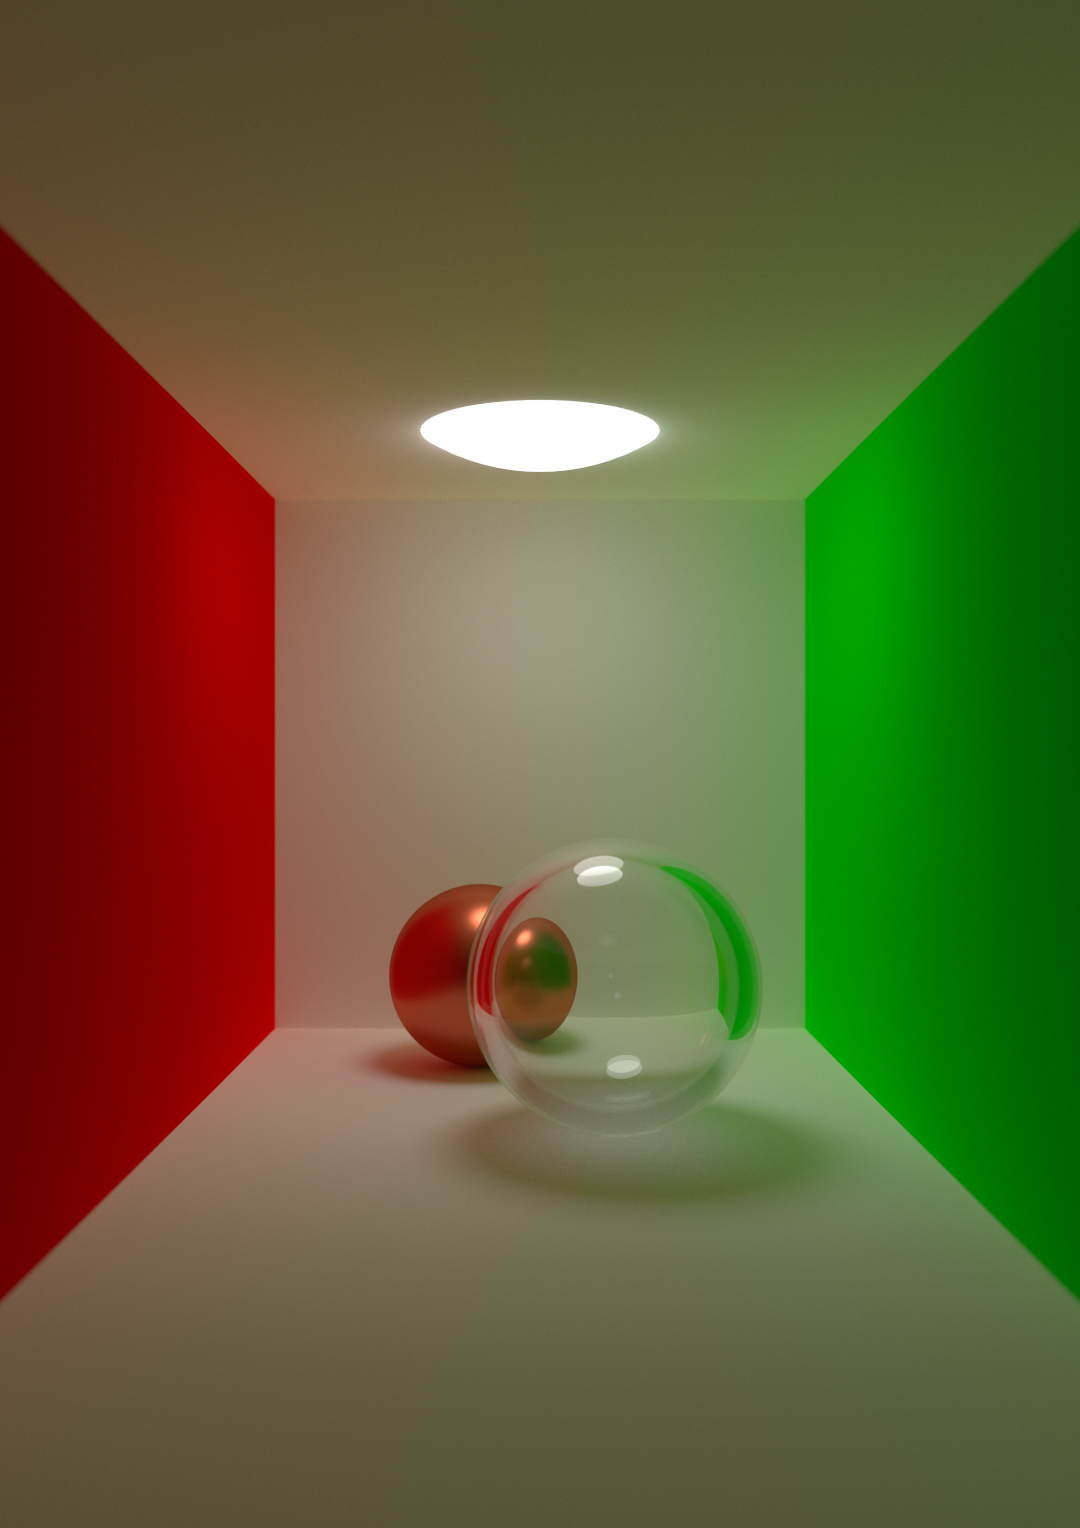
\includegraphics[width=\linewidth]{images/blender_out_small.png}
    Blender
\end{minipage}
\hspace{0.5cm}
\begin{minipage}[b]{0.45\linewidth}
    \centering
    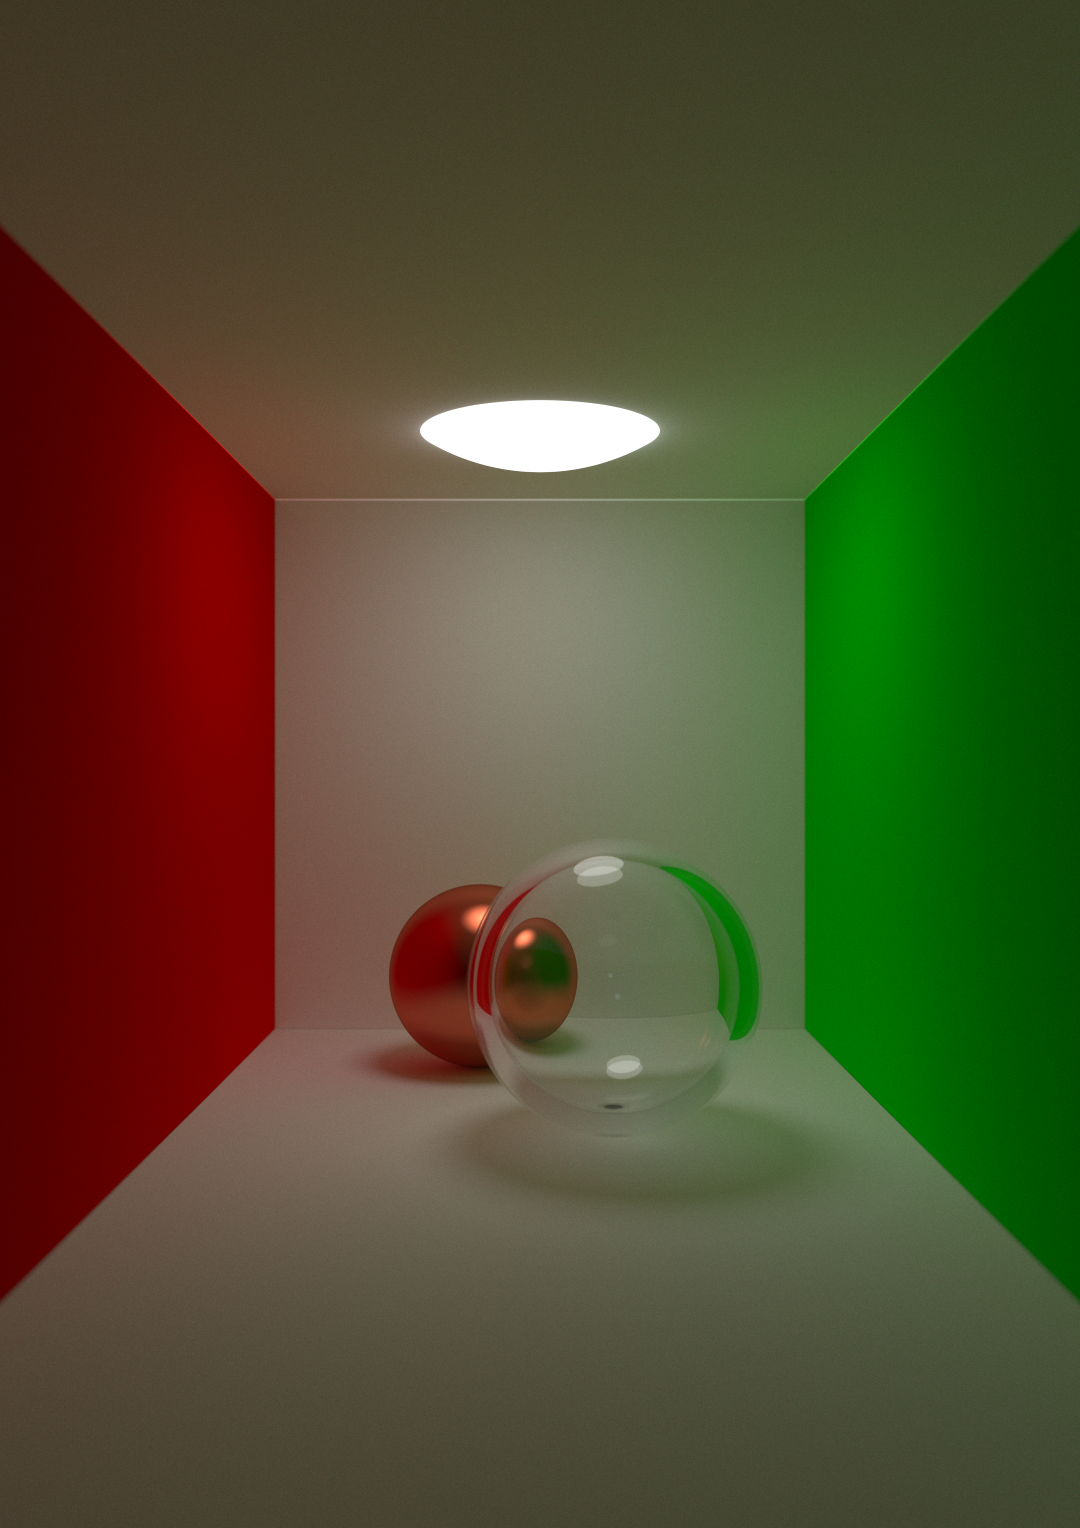
\includegraphics[width=\linewidth]{images/out_small.png}
    Eigenes Programm
\end{minipage}
\end{center}

Um zu überprüfen, ob das Programm korrekt funktioniert, wurde ein Vergleich mit Blender durchgeführt.
Dazu wurde eine Szene im eigenen Programm erstellt und in Blender nachgebaut.
Die Szene ist eine Cornell-Box mit einer metallisch glänzenden Kugel und einer hohlen Glaskugel.
Die Lichtquelle ist eine Kugel in der Decke der Box.
Beide Bilder wurden mit einer Auflösung von 4094x5793 Pixeln, 1024 Samples pro Pixel und 24 Bounces pro Sample gerendert.
Die Renderzeit betrug ca. 4 Stunden für das eigene Programm und 23 Minuten für Blender.
Beide Bilder sind ähnlich verrauscht.

Es können einige Unterschiede zwischen den Bildern festgestellt werden:
In Blender können bei der beleuchtenden Kugel die Flachen Kanten der Polygone gesehen werden, während im eigenen Programm die Kugel glatt erscheint.
Am Berührungspunkt der Glaskugel mit dem Boden ist im eigenen Programm ein schwarzer Punkt zu sehen, der in Blender nicht vorhanden ist.
Im eigenen Programm sind außerdem die oberen Kanten der Box unnatürlich hell.
Insgesamt ist das Blender Bild etwas heller als das eigene, beide sind aber ähnlich genug, um zu sagen, dass das Programm funktioniert.

Beim Erstellen der Szene in Blender ist aufgefallen, dass das eigene Programm Bilder spiegelverkehrt rendert.
Um die Bilder zu vergleichen, wurde die Szene in Blender spiegelverkehrt aufgebaut.

\printbibliography[heading=bibintoc, title=Quellen]
Die Ausarbeitung wurde mit \LaTeX{} erstellt, unter Verwendung von Github Copilot.
\end{document}